%Empieza configuracion de capitulo
\setstretch{1.0}
\titleformat{\chapter}[block]{\Large\bfseries}{CHAPTER \Huge\thechapter\vspace{25 pt}}{0 pt}{\\\fontsize{26}{36}\selectfont}
\titlespacing{\chapter}{0 pt}{30 pt}{50 pt}[0 pt]
\titleformat{\section}{\Large\bfseries}{\thesection}{0 pt}{\hspace{30 pt}}
\titleformat{\subsection}{\large\bfseries}{\thesubsection}{0 pt}{\hspace{30 pt}}
\pagestyle{fancy}
\fancyhead[LO,LE]{\footnotesize\emph{\leftmark}}
\fancyhead[RO,RE]{\thepage}
\fancyfoot[CO,CE]{}
%Termina configuracion de capitulo

\chapter{System Architecture}
\setstretch{1.5} %Regresa el interlineado a 1.5

\normalsize
\noindent
In this chapter it is described the architecture of the embedded system
employed in this work. It is provided a hardware and software description.
It also includes an explanation of the MPI implementation utilized 
use. At the end, it is presented the description of the implemented topology of
the system.

\section{Selected Embedded System}
\noindent

\subsection{Development Board} The development board utilized to perform
experiments is a MinnowBoard MAX \cite{minnowboard} and it has a processor
Intel Atom-TM Processor E3825 \textregistered\ \cite{E3825}. The main characteristics are
described in Table~\ref{tab:4.1}:

    \begin{figure}[H]
        \centering
        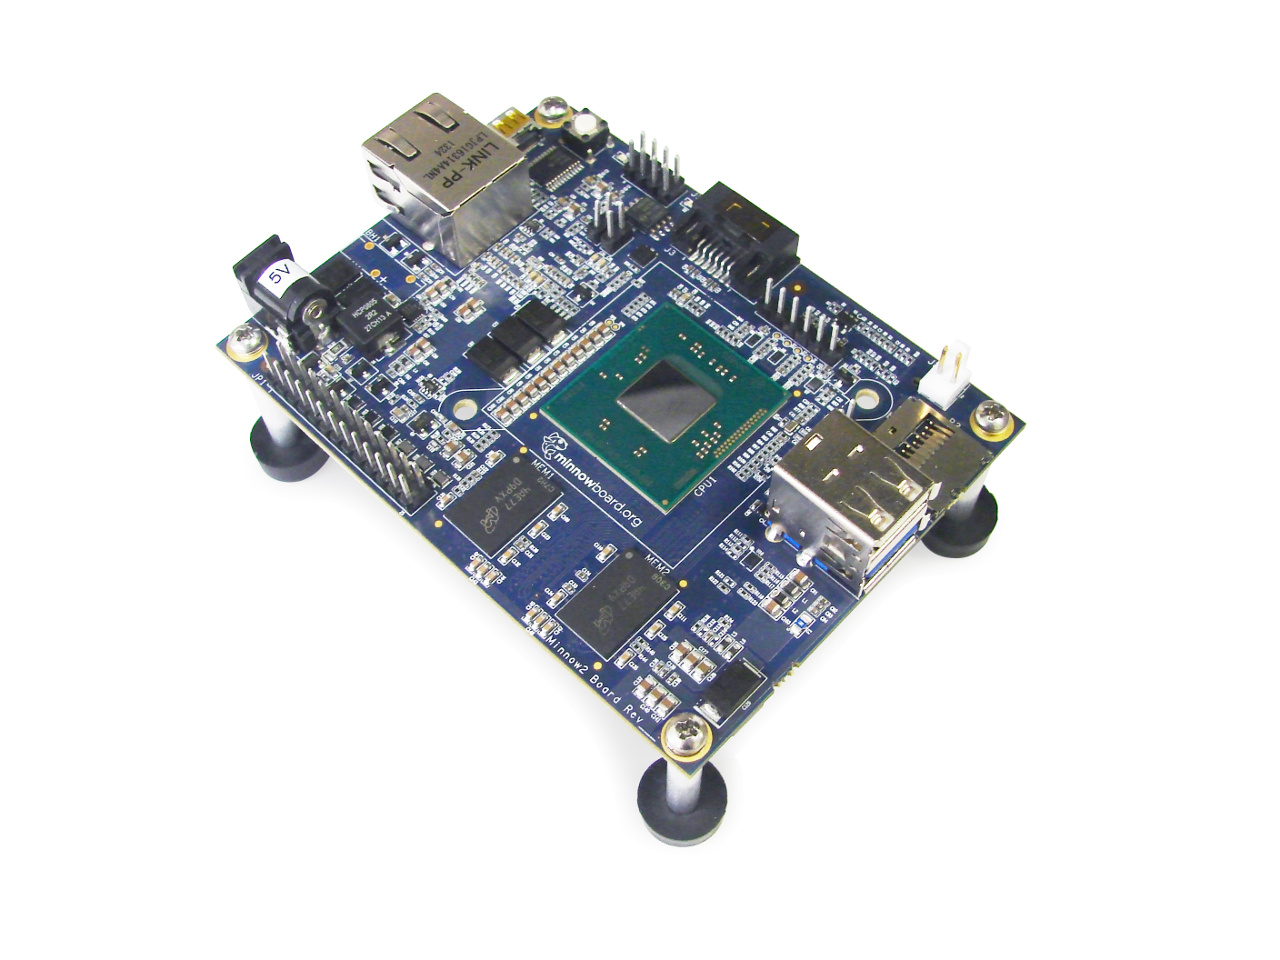
\includegraphics[width=0.75\textwidth]{images/minnow-max.jpg}.png
        \caption{Minnow board max platform}
        \label{fig:4.1}
    \end{figure}


    \begin{figure}[H]
        \centering
        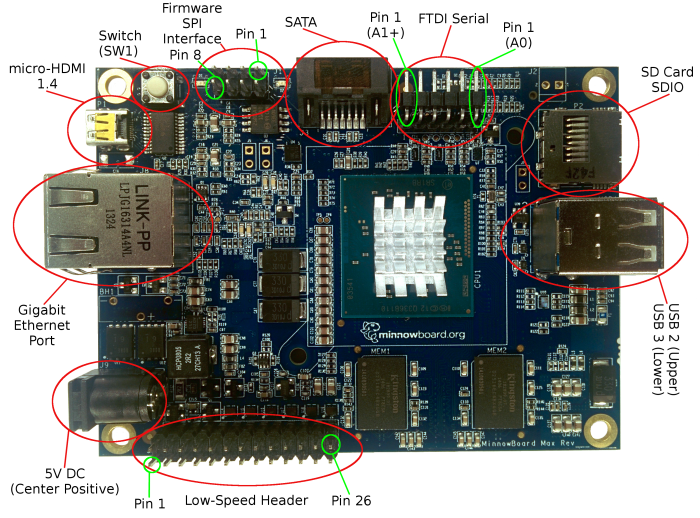
\includegraphics[width=0.75\textwidth]{images/minnow-max-2.png}
        \caption{Connection ports of the  MinnowBoard MAX}
        \label{fig:4.2}
    \end{figure}

    \begin{center}
    \begin{tabular}{ | l | r |}
        \hline
        Processor Number & E3825  \\ \hline
        \# of cores & 2  \\ \hline
        \# of Thread & 2  \\ \hline
        Clock Speed & 1.3 GHz  \\ \hline
        L2 Cache & 1MB  \\ \hline
        Instruction Set & 64 bit  \\ \hline
    \end{tabular}
    \captionof{table}{Intel\textregistered\  Atom Processor E3825
    Specifications} \label{tab:4.1}
    \end{center}

Figure~\ref{fig:4.1} and ~\ref{fig:4.2} shows pictures of the MinnowBoard MAX.
It is a development platform for both professionals and entrepreneurs. The
MinnowBoard MAX is an open hardware platform: anyone can have access to see the
source design and documentation, can study it, modify it and share it.

\subsection{Embedded Operating System} 

Typical embedded system does not contain an operating system (usually); but due
to the complexity of current embedded applications is plenty necessary to have
an operating system that manage all the processes that current embedded
applications have. 

To perform the experiments on the selected board, it was decided to include a
full operating system running. It includes a boot manager, a full file system ,
kernel and user spaces. According to \cite{minnowboard} the board supports
multiple kind of operating systems. In this work three different, Linux-based,
operating systems:

\begin{itemize}
    \item Fedora \cite{fedora}
    \item Clear Linux for Intel Architecture \cite{clear-linux}
    \item Yocto \cite{yocto-project}
\end{itemize}

The work performs a comparison between the three. There are multiple 
configurations for each one, such that the performance of implemented embedded
cluster behaves differently. 

\subsection{Embedded Firmware}

The  MinnowBoard MAX  board is a low-cost, commercially available, reference
platform for hardware, software and firmware developers who wish to work with
an open design development environment. Its design specifications
and materials have been provided to the open community for the purpose of
enabling experimentation and development of technical solutions based upon
the  MinnowBoard MAX board.

The download page presents firmware components for the reference board. For
this work were downloaded the official BIOS Firmware Binary Images
\cite{minnowmax-firmware}.

\section{Selected Traditional Computing System}
\noindent

The selected traditional computing system we chose is the Intel NUC D54250WYK
platform. As we can see in \cite{Bo} and \cite{Shen} this kind of platforms are
used as media centers and cloud system for heterogeneous sensors. This part
will describe hardware of the development board as well as the software we are
going to use (operating system and firmware).

\subsection{Development Board} 

The platform we will use for our experiment is the
Intel\textregistered\ NUC D54250WYK Their main characteristics are
described in Table~\ref{tab:4.2} \cite{NUC}.

    \begin{center}
    \begin{tabular}{ | l | r |}
        \hline
        Processor Number & Intel Core™ i5-4250U Processor \\ \hline
        \# of cores &  2 \\ \hline
        \# of Thread & 4  \\ \hline
        Clock Speed & 1.3 GHz  \\ \hline
        L2 Cache & 3MB  \\ \hline
        Instruction Set & 64 bit  \\ \hline
    \end{tabular}
    \captionof{table}{Intel\textregistered\ NUC D54250WYK Specifications} \label{tab:4.2}
    \end{center}


\subsection{Operating System} 

The board support multiple kind of Operating Systems. In \cite{NUC-OS} there is
a list of available operating systems to install. However, due to the good
performance results \cite{phoronix-clear} we are going to use the Clear Linux
project for Intel architecture \cite{clear-linux}. The Clear Linux Project for
Intel\textregistered\ Architecture is a project that is building a Linux OS
distribution for various cloud use cases. The goal of Clear Linux OS is to
showcase the best of Intel Architecture technology, from low-level kernel
features to more complex items that span across the entire operating system
stack.


\section{Studied Network Topologies}

In computer networking, topology refers to the layout of connected devices. This
section describes standard topologies of networking.

According to \cite{topologies-intro} \textit{"In networking a topology is a
virtual shape or structure. This shape does not necessarily correspond to the
actual physical layout of the devices on the network"}. For example, the
computers on a home network may be arranged in a circle in a family room, but
it would be highly unlikely to find a ring topology there.

According to \cite{topologies-intro} network topologies are categorized into
the following basic types:

\begin{itemize}
    \item Bus
    \item Ring
    \item Star
    \item Tree
    \item Mesh
\end{itemize}

More complex networks can be built as hybrids of two or more of the above basic
topologies.

For the experiments of this work it is utilized the star topology (see
Figure~\ref{fig:4.3}). According to \cite{star-top} \textit{ "In a star topology
, each device on the network connects to a centralized device via a single
cable. This arrangement creates a point to point network connection between the
two devices and overall gives the appearance of a star"}.

The network does not necessarily have to have the appearance of a star to be
classified as a star network, but all of the nodes on the network must be
connected to one central device. Because each device must have its own cable, a
star topology requires far more able than other topologies.

The star topology is considered the easiest topology to design and implement.
One of the biggest advantages of the star topology is that computers can be
connected to and disconnected without affecting the other systems. However, in
the star topology, all devices on the network connect to  central device, and
this central device creates a single point of failure on the network
\cite{star-top}.

\begin{figure}[H]
\centering
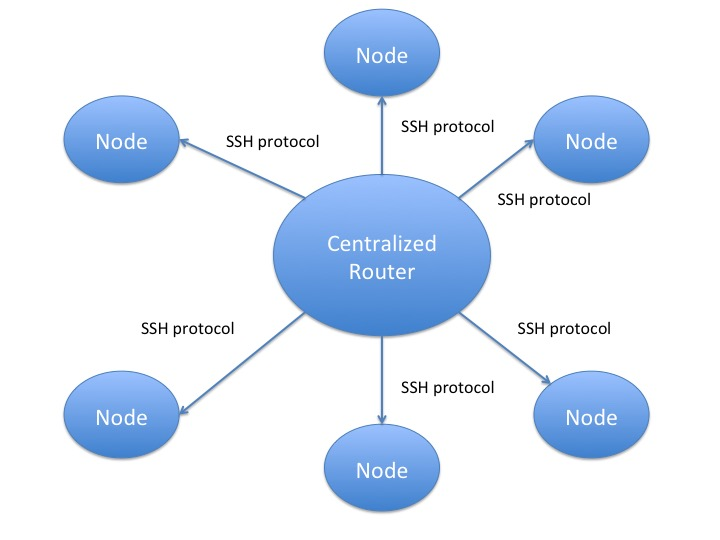
\includegraphics[width=1\textwidth]{images/star_topology.png}
\caption{Star topology diagram}
\label{fig:4.3}
\end{figure}


\section{Architecture Diagram}

Figure~\ref{fig:4.4} shows the diagram of the architecture of the embedded
cluster employed in this research work in an star topology. 

\begin{figure}[H]
\centering
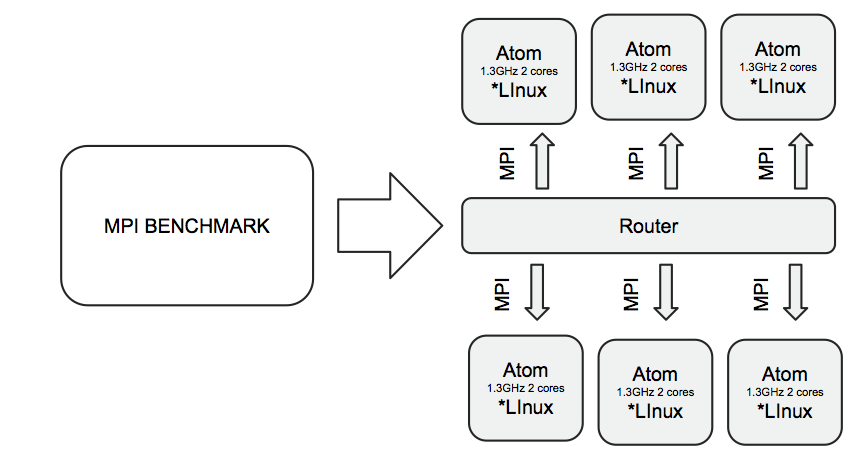
\includegraphics[width=1\textwidth]{images/cluster_minnows.png}
\caption{System architecture diagram }
\label{fig:4.4}
\end{figure}

\noindent

\clearpage
